\documentclass{article}

\usepackage{fullpage}
\usepackage{graphicx}

\title{A review of steer torque measurements in bicycles and motorcycles}
\author{Jason K. Moore, P. D. L de Lange and Mont Hubbard}
\date{\today}

\begin{document}

\maketitle

Applying forces to the handlebars of motorcycles and bicycles which result in a
net torque between the front frame and the rear frame (and rider) about the
steer axis provide the most authority of any other input for control of the
lateral dynamics of the vehicles. It is also clear that haptic feedback is very
important and maybe essential for a human to balance a bicycle or motorcycle.
Thus is it critical to understand how the steer torque plays a role in both the
open loop and closed loop dynamics of the bicycle/motorcycle-rider system.

The first portion of the paper will be devoted to a review of steer torque
measurements and modeling results. For example, the earliest measurements of
steer torque were done on a motorcycle by \cite{Wilson-Jones1951} with a manual
scale. There have since various sensors designed to measure steer torque that
have various degrees of range and accuracy.

The applied steer torque needed to control a motorcycle is generally much
greater in magnitude for that of a bicycle. For similar manuevers motorcycles
may require up to 50 Nm while bicycles require up to 10 Nm. Furthermore, the
rider can easily apply forces and moments to the handlebars which are up 20
times larger in magnitude than the steer torque. The sensors must me designed
such that these other forces do not corrupt the much lower magintued steer
torque measurements.

There are several types of designs for measuring steer torque: force
transducers at the hand-handlebar interface, torque transducers on or in the
steer tube, and variations of secondary handlebars connected through
transducers. The merits of each type of design is discussed in the paper.

We show that careful attention must be made to any steer torque sensors which
measure the strain at points between the hands and the front wheel contact point.
Depending on the location along the steer axis that the measurement is made,
the interial effects of front frame and handlebars between the sensor and the
rider's hands must be accounted for. For bicycles, this is very important
because the torques due to the inerital effects can be a high percentage of the
actual applied torque. No previous steer torqe measurements seem to take this
into account.

\begin{figure}
  \centering
  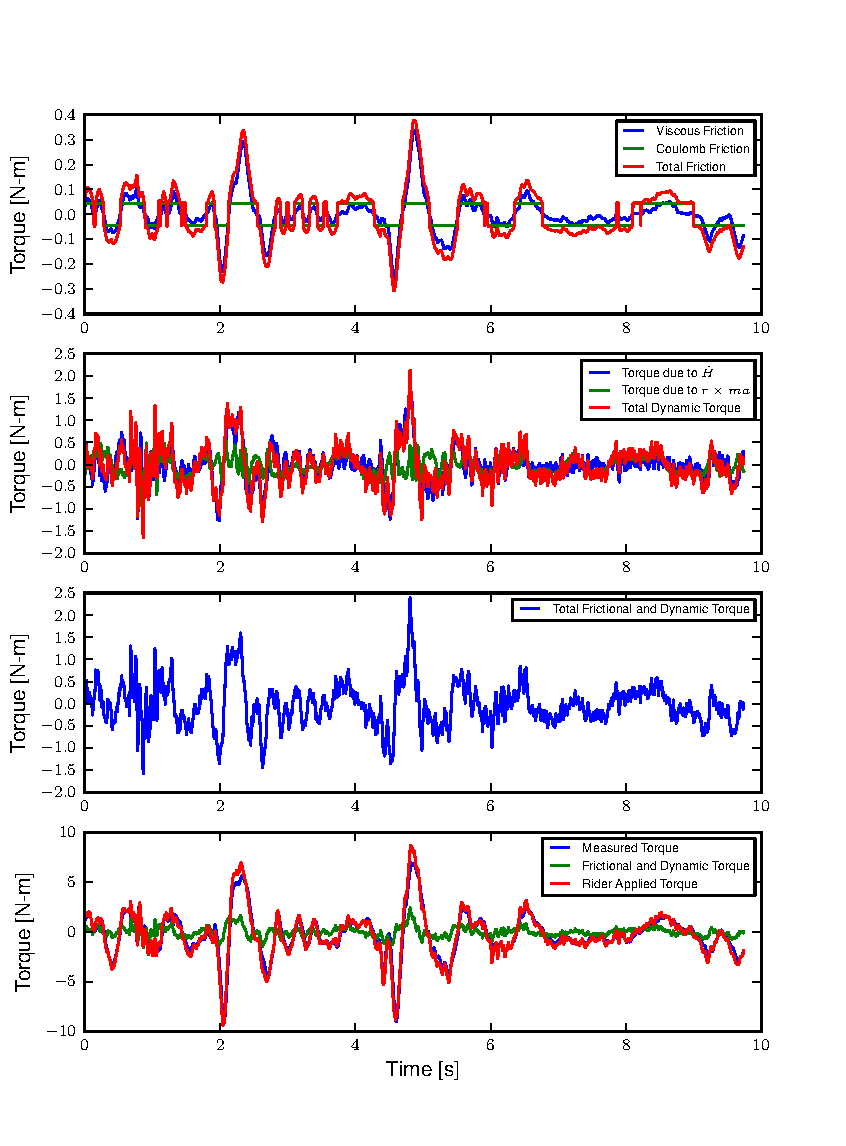
\includegraphics[width=5.0in]{steer-torque-components.pdf}
  \caption{This is a plot of the steer torque components for run \#700. The top
  plot shows the additive viscous and Coulomb friction. The total bearing
  friction during the run is less 0.3 Nm. The second plot shows the torque the
  rider must apply to overcome the handlebar inertia. The dominant term is the
  $I_{G_{33}} w_{b3}$ and during the peak accelerations the additive torque is
  up to 1.5 Nm for this run. The third plot shows the total additive torque
  which is up to 2 Nm. And finally the last plot shows the difference in the
  measured torque and the rider applied torque. There are large differences,
  especially at the peaks.}
\end{figure}

Finally, we will show the steer torque measurement sensor designed for an
instrumented bicycle which attempts to take into account many of the flaws of
previous measurements. We include experimental results measuring headset
bearing friction and we show results for very accurate torque measurements in
various bicycle manuevers giving qualitative look at typical steer torque
measurements.

This paper is based on work supported by the National Science Foundation under
Grant No 0928339.

\bibliographystyle{plain}
\bibliography{bicycle}

\end{document}
